\documentclass[UTF8]{ctexart}
\usepackage{amsmath}
\usepackage{amssymb}
\usepackage{background}
\usepackage{booktabs}
\usepackage{caption}
\usepackage{enumitem}
\usepackage{graphicx}
\usepackage{geometry}
\usepackage{float}
\usepackage{fontspec}
\usepackage{mathptmx} %mathptmx和times结合使得公式使用times new roman字体
\usepackage{pifont}
\usepackage{tikz}
\usepackage{times}
\usepackage{xcolor}
\usetikzlibrary{positioning, arrows.meta, shapes.misc}



\geometry{a5paper, top=0.1cm, left=1cm, right=1cm, bottom=1cm, footskip=0.3cm, marginparsep=0.1cm}
\setCJKmainfont[BoldFont={汉仪文黑-85W},ItalicFont={方正苏新诗柳楷简体}]{汉仪文黑-55W}
\setfontfamily\Issue{Century Schoolbook}
\newCJKfontfamily\TitleFont{思源宋体 CN Heavy}
\newfontfamily\timesnewroman{Times New Roman}
\setmainfont{Times New Roman}
\captionsetup{font=small, labelfont=bf}
\colorlet{backcolor}{yellow!80!gray!20!} %若只有两页以内,可删去
\pagecolor{backcolor}

\CTEXsetup[format = {\centering\bfseries\normalsize}, beforeskip = 0pt, afterskip = 0pt]{section}

\newcommand\Black[1]{\textcolor[gray]{0.3}{#1}}
\newcommand\Brown[1]{\textcolor[HTML]{998A4E}{#1}}
\newcommand\Emph[1]{\colorbox{red!20!}{\textcolor{red!80!black}{#1}}}
\newcommand\Correct[1]{\colorbox{green!20}{\textcolor{green!50!black}{#1}}}
\newcommand\Mathemph[1]{\text{\textcolor{green!60!black}{$#1$}}}
\newcommand\Concept[1]{\colorbox{cyan!10!white}{\textcolor{cyan!40!black}{#1}}}
\newcommand\Notes[1]{\textcolor{yellow!50!black}{\small #1}}
\newcommand\Example[1]{\textcolor{cyan!70!black}{\small #1}}
\newcommand\relation[2]{\langle #1,#2 \rangle}
\newcommand\pos[1]{\marginpar{\footnotesize\ttfamily\textcolor{yellow!50!black}{\hfill #1}}}

\newcommand\h{\text{\textcolor{blue}{\,$\wedge$\,}}} %合取
\newcommand\x{\text{\textcolor{red!70!black}{\,$\vee$\,}}} %析取
\newcommand\f{\neg} %非
\newcommand\is{\Leftrightarrow\ } %等价
\newcommand\defines{:=}

%这4个信息随“刊号”更新
\newcommand\IssueNumber{07}
\newcommand\Date{2023-10-31}
%\newcommand\Contributer{@金光日}
\newcommand\Subject{离散数学}


\begin{document}
\backgroundsetup{contents=\includegraphics{示例.png}, center, scale=1, angle=0, opacity=1}
\BgThispage
\begin{center}
{\scriptsize\Issue \textcolor[HTML]{C8BA83}{WEEKLY TIPS}}

{\Huge\bfseries\TitleFont \Black{知\ 识\ 小\ 料}}

\vspace{-0.1cm}
{\footnotesize \Brown{「电计 2203 班」周常规知识整理共享}}
\end{center}

\vspace{-0.5cm}

\begin{figure}[H]
\hspace{1cm}
\begin{minipage}[t]{0.3\textwidth}
\centering
    \Brown{ISSUE.}

    \vspace{-0.6cm}
    \Huge \Issue\slshape\bfseries\Black{\IssueNumber}
\end{minipage}
\hfill
\begin{minipage}[t]{0.3\textwidth}
\centering
    \Brown{日期:\Date} \\
%\vspace{-0.1cm}
%    \Brown{贡献者:\Contributer} \\
\vspace{-0.1cm}
    \Brown{学科:\Subject} \\
\end{minipage}
\vspace{-0.2cm}
\end{figure}

\begin{center}\color{cyan!50!black}
设 $A=\{1,2,3,4\}$,$A$ 上关系 $R$ 如下图,则 $R^2=$\underline{\hspace{2cm}}。

\begin{figure}[htb]
    \centering
    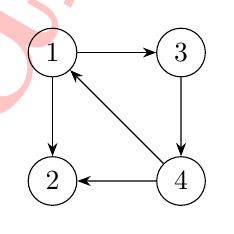
\begin{tikzpicture}[->, >=Stealth, scale=0.8]
        \node[draw,circle] (A) {1};
        \node[draw,circle] (B) [below = of A] {2};
        \node[draw,circle] (C) [right = of A] {3};
        \node[draw,circle] (D) [below = of C] {4};
        \draw (A) -- (B);
        \draw (A) -- (C);
        \draw (C) -- (D);
        \draw (D) -- (A);
        \draw (D) -- (B);
    \end{tikzpicture}
\end{figure}
\end{center}

\vspace{-0.8cm}
可以由关系图写出关系 
\begin{equation*}
    R = \{\relation{1}{2}, \relation{1}{3}, \relation{3}{4}, \relation{4}{1}, \relation{4}{2}\}
\end{equation*}
再用关系乘积的定义计算 $R^2$ 即 $R*R$,易得 $R^2 = \{\relation{1}{4}, \relation{3}{1}, \relation{3}{2}, \relation{4}{2}, \relation{4}{3}\}$。这是常规方法,但是对关系乘积还可以有新的理解方式。

我们可以把关系乘积理解为一个\Emph{「抄近路」}的过程。对于「$A\to B$」和「$B\to C$」的两条路线,由于 $B$ 是共同的中转点,因此可以抄一条近路,直接从 $A$ 一步到 $C$。举个例子,\textcolor{green!50!black}{$S=\{\relation{\text{综一}}{\text{中食}}\}$,$T=\{\relation{\text{中食}}{\text{寝室}}\}$},可以理解为两条路,一条从综一到中食,另一条从中食到寝室,抄近路可以从综一直达寝室,也就是 \textcolor{green!50!black}{$S*T = \{\relation{\text{综一}}{\text{寝室}}\}$}。

\begin{figure}[htb]
  \centering
  \begin{tikzpicture}[>=Stealth, point/.style={rounded rectangle, top color=white, bottom color=cyan!20, draw=cyan!70!black, thick}]
        \node[draw, point] at (0,0) (A) {综一};
        \node[draw, point] at (2,1) (B) {中食};
        \node[draw, point] at (4,0) (C) {寝室};
        \draw[->] (A) -- (B) node[above,midway] {$S$};
        \draw[->] (B) -- (C) node[above,midway] {$T$};
        \draw[->, blue] (A) -- (C) node[above,midway] {$S*T$};
  \end{tikzpicture}
\end{figure}

那么回到原题,我们可以发现存在 $1\to 3\to 4$ 的路径,可以「抄近路」得到 $1\to 4$,也就是 $R^2$ 里面有一个有序对 $\relation{1}{4}$。类似的,还有 $3\to 4\to 1$、$3\to 4\to 2$、$4\to 1\to 2$、$4\to 1\to 3$ 等路径,各自「抄近路」即可得到剩余的有序对。

\vspace{0.2cm}

\textcolor{cyan!80!black}{【结论】$\{\relation{1}{4}, \relation{3}{1}, \relation{3}{2}, \relation{4}{2}, \relation{4}{3}\}$。}

\textcolor{cyan!80!black}{【点评】本题是一道求关系乘积(关系复合)的题目,难度简单,但从另一个角度理解和分析,或许会有新的收获……}


%\newpage
%\backgroundsetup{contents=\includegraphics{下半示例.png}, center, scale=1, angle=0, opacity=1}
%\phantom{...}
%\vspace{0.3cm}
%\BgThispage
%
%{\color{cyan!50!black}
%第二题:设代数系统 $\relation{A}{\oplus}$,其中 $A=\{a,b,c\}$,则幺元是\underline{\hspace{2cm}};是否有等幂性\underline{\hspace{2cm}};是否有对称性\underline{\hspace{2cm}}。
%
%\begin{table}[htb]
%\centering
%\color{cyan!50!black}
%\begin{tabular}{c|ccc}
%    \toprule
%    $\oplus$ & $a$ & $b$ & $c$ \\
%    \midrule
%    $a$ & $a$ & $b$ & $c$ \\
%    $b$ & $b$ & $b$ & $c$ \\
%    $c$ & $c$ & $c$ & $b$ \\
%    \bottomrule
%\end{tabular}
%\end{table}
%}
%
%\begin{itemize}[itemsep=0pt, parsep=0pt]
%  \item $e$ 是幺元——对任意集合中的 $x$,总有 $x\oplus e=e\oplus x=x$;
%  \item 等幂性——对任意集合中的 $x$,总有 $x\oplus x=x$;
%  \item 对称性——其实就是 $\oplus$ 的交换律。
%\end{itemize}
%
%因此观察运算表,$a$ 所在行的三个表项分别为 $a,b,c$,这与行表头一致(也就是 $a\oplus a=a$,$a\oplus b=b$,$a\oplus c=c$),因此 $a$ 是左幺元。$a$ 所在列也同理,因此 $a$ 是右幺元。左右都满足,因此称 $a$ 是幺元。由幺元的唯一性,$b,c$ 均不是幺元。\textcolor{cyan}{(进一步可发现,这个代数系统不存在零元。)}
%
%要判断等幂性,不难发现 $c\oplus c=b$,因此不满足。
%
%要判断对称性,可以看是否满足交换律。可发现 $a\oplus b = b\oplus a$,$a\oplus c=c\oplus a$,$b\oplus c=c\oplus b$,穷举所有三种可能,发现满足交换律。







\end{document} 